\documentclass{article}
\usepackage{tikz}
\usetikzlibrary{arrows.meta}
\usepackage[margin=0.5cm, paperwidth=10cm, paperheight=8cm]{geometry} % Adjust the paper size 

\begin{document}
\thispagestyle{empty} % Remove page numbers

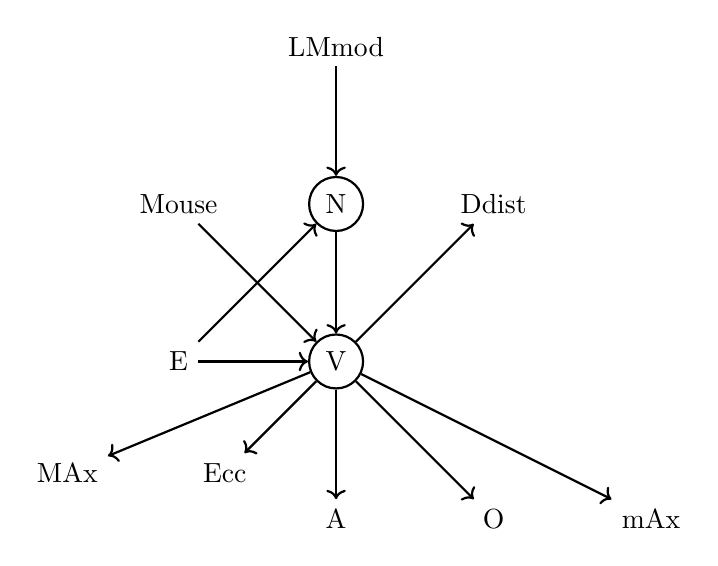
\begin{tikzpicture}[node distance=2cm, thick]

    % Nodes
    \node (V) [circle, draw] {V};
    \node (N) [circle, draw, above of=V] {N};
    \node (E) [left of=V] {E};
    \node (Mouse) [left of=N] {Mouse};
    \node (LMmod) [above of=N] {LMmod};
    \node (Ddist) [right of=N] {Ddist};
    
    % Other labels below V
    \node (Ecc) [below left of=V] {Ecc};
    \node (MAx) [left of=Ecc] {MAx};
    \node (A) [below of=V] {A};
    \node (O) [right of=A] {O};
    \node (mAx) [right of=O] {mAx};

    % Arrows
    \draw[->] (LMmod) -- (N);
    \draw[->] (Mouse) -- (V);
    \draw[->] (N) -- (V);
    \draw[->] (V) -- (Ddist);
    \draw[->] (E) -- (V);
    \draw[->] (E) -- (N);

    \draw[->] (V) -- (MAx);
    \draw[->] (V) -- (Ecc);
    \draw[->] (V) -- (A);
    \draw[->] (V) -- (O);
    \draw[->] (V) -- (mAx);

\end{tikzpicture}

\end{document}
